%%%%%%%%%%%%%%%%%%%%%%%%%%%%%%%%%%%%%%%%%
% Masters/Doctoral Thesis 
% LaTeX Template
% Version 1.43 (17/5/14)
%
% This template has been downloaded from:
% http://www.LaTeXTemplates.com
%
% Original authors:
% Steven Gunn 
% http://users.ecs.soton.ac.uk/srg/softwaretools/document/templates/
% and
% Sunil Patel
% http://www.sunilpatel.co.uk/thesis-template/
%
% License:
% CC BY-NC-SA 3.0 (http://creativecommons.org/licenses/by-nc-sa/3.0/)
%
% Note:
% Make sure to edit document variables in the Thesis.cls file
%
%%%%%%%%%%%%%%%%%%%%%%%%%%%%%%%%%%%%%%%%%

%----------------------------------------------------------------------------------------
%	PACKAGES AND OTHER DOCUMENT CONFIGURATIONS
%----------------------------------------------------------------------------------------

\documentclass[11pt, oneside]{Thesis} % The default font size and one-sided printing (no margin offsets)

\graphicspath{{../graphics/}} % Specifies the directory where pictures are stored

\usepackage[square, numbers, comma, sort&compress]{natbib} % Use the natbib reference package - read up on this to edit the reference style; if you want text (e.g. Smith et al., 2012) for the in-text references (instead of numbers), remove 'numbers' 

%from my usual papers
\usepackage{amsmath}
\usepackage{amssymb}
\usepackage{amsthm}
\usepackage{amscd}
\usepackage{amsfonts}
\usepackage{graphicx}%
%\usepackage{fancyhdr}
%\usepackage{color}
%\usepackage{cite}
\usepackage{physics}
\usepackage{float}
\usepackage{caption}
\usepackage{subcaption}

\hypersetup{urlcolor=blue, colorlinks=true} % Colors hyperlinks in blue - change to black if annoying
\title{\ttitle} % Defines the thesis title - don't touch this

\begin{document}

\frontmatter % Use roman page numbering style (i, ii, iii, iv...) for the pre-content pages

\setstretch{1.3} % Line spacing of 1.3

% Define the page headers using the FancyHdr package and set up for one-sided printing
\fancyhead{} % Clears all page headers and footers
\rhead{\thepage} % Sets the right side header to show the page number
\lhead{} % Clears the left side page header

\pagestyle{fancy} % Finally, use the "fancy" page style to implement the FancyHdr headers

\newcommand{\HRule}{\rule{\linewidth}{0.5mm}} % New command to make the lines in the title page

%code handling
\newcommand{\raven}{\texttt{RAVEN}}
\newcommand{\bison}{\texttt{BISON}}
\newcommand{\moose}{\texttt{MOOSE}}

% some handy math stuff
\newcommand{\expv}[1]{\ensuremath{\mathbb{E}[ #1]}}
\newcommand{\xs}[2]{\ensuremath{\Sigma_{#1}^{(#2)}}}
\newcommand{\intO}{\ensuremath{\int\limits_{4\pi}}}
\newcommand{\intz}{\ensuremath{\int\limits_0^1}}
\newcommand{\intf}{\ensuremath{\int\limits_{-\infty}^\infty}}
\newcommand{\intzf}{\ensuremath{\int\limits_{0}^\infty}}
\newcommand{\LargerCdot}{\raisebox{-0.25ex}{\scalebox{1.2}{$\cdot$}}}
\newcommand{\hold}[1]{\ensuremath{\Big|_{#1}}}

\renewcommand{\vec}[1]{\mathbf{#1}}

% PDF meta-data
\hypersetup{pdftitle={\ttitle}}
\hypersetup{pdfsubject=\subjectname}
\hypersetup{pdfauthor=\authornames}
\hypersetup{pdfkeywords=\keywordnames}

%----------------------------------------------------------------------------------------
%	TITLE PAGE
%----------------------------------------------------------------------------------------

\begin{titlepage}
\begin{center}

\textsc{\LARGE \univname}\\[1.5cm] % University name
\textsc{\Large Doctoral Thesis}\\[0.5cm] % Thesis type

\HRule \\[0.4cm] % Horizontal line
{\huge \bfseries \ttitle}\\[0.4cm] % Thesis title
\HRule \\[1.5cm] % Horizontal line
 
\begin{minipage}{0.4\textwidth}
\begin{flushleft} \large
\emph{Author:}\\
%\href{http://www.johnsmith.com}
{\authornames} % Author name - remove the \href bracket to remove the link
\end{flushleft}
\end{minipage}
\begin{minipage}{0.4\textwidth}
\begin{flushright} \large
\emph{Supervisor:} \\
%\href{http://www.jamessmith.com}
{\supname} % Supervisor name - remove the \href bracket to remove the link  
\end{flushright}
\end{minipage}\\[3cm]
 
\large \textit{Submitted in partial fulfilment of the requirements\\ for the degree of \degreename}\\[0.3cm] % University requirement text
\textit{in the}\\[0.4cm]
%\groupname\\
\deptname\\[2cm] % Research group name and department name
 
{\large \today}\\[4cm] % Date
%\includegraphics{Logo} % University/department logo - uncomment to place it
 
\vfill
\end{center}

\end{titlepage}

%----------------------------------------------------------------------------------------
%	DECLARATION PAGE
%	Your institution may give you a different text to place here
%----------------------------------------------------------------------------------------

%\Declaration{
%
%\addtocontents{toc}{\vspace{1em}} % Add a gap in the Contents, for aesthetics
%
%I, \authornames, declare that this thesis titled, '\ttitle' and the work presented in it are my own. I confirm that:
%
%\begin{itemize} 
%\item[\tiny{$\blacksquare$}] This work was done wholly or mainly while in candidature for a research degree at this University.
%\item[\tiny{$\blacksquare$}] Where any part of this thesis has previously been submitted for a degree or any other qualification at this University or any other institution, this has been clearly stated.
%\item[\tiny{$\blacksquare$}] Where I have consulted the published work of others, this is always clearly attributed.
%\item[\tiny{$\blacksquare$}] Where I have quoted from the work of others, the source is always given. With the exception of such  quotations, this thesis is entirely my own work.
%\item[\tiny{$\blacksquare$}] I have acknowledged all main sources of help.
%\item[\tiny{$\blacksquare$}] Where the thesis is based on work done by myself jointly with others, I have made clear exactly what was done by others and what I have contributed myself.\\
%\end{itemize}
% 
%Signed:\\
%\rule[1em]{25em}{0.5pt} % This prints a line for the signature
% 
%Date:\\
%\rule[1em]{25em}{0.5pt} % This prints a line to write the date
%}

\clearpage % Start a new page

%----------------------------------------------------------------------------------------
%	QUOTATION PAGE
%----------------------------------------------------------------------------------------

\pagestyle{empty} % No headers or footers for the following pages

%\null\vfill % Add some space to move the quote down the page a bit
%
%\textit{``Thanks to my solid academic training, today I can write hundreds of words on virtually any topic without possessing a shred of information, which is how I got a good job in journalism."}
%
%\begin{flushright}
%Dave Barry
%\end{flushright}
%
%\vfill\vfill\vfill\vfill\vfill\vfill\null % Add some space at the bottom to position the quote just right
%
%\clearpage % Start a new page

%----------------------------------------------------------------------------------------
%	ABSTRACT PAGE
%----------------------------------------------------------------------------------------

\addtotoc{Abstract} % Add the "Abstract" page entry to the Contents

\abstract{\addtocontents{toc}{\vspace{1em}} % Add a gap in the Contents, for aesthetics

As the complexity of experiments in fields such as nuclear engineering continues to increase, so too does the
demand for robust computational methods to simulate these experiments in virtual space.  In many of these
simulations, exact input design parameters as well as intrinsic properties of the experiment are often sources
of input uncertainty.  Often, small perturbations in these uncertain parameters have significant impact on the
outcome of an experiment.  For instance, when considering nuclear fuel performance experiments, small changes
in the thermal conductivity of the fuel can greatly affect the maximum stress on the surrounding cladding.  In
recent years quantifying the impact of the input uncertainties in such an experimental system has grown as the
complexities in these systems increase.  For some problems, the input parametric space and corresponding
quantity of interest output space is sufficiently explored with a few low-cost computational calculations.
For others, however, the computational model is costly and it takes a great many random samples to obtain a
good understanding of the output space.  This research explores the possibilities of advanced methods in
stochastic collocation for generalized polynomial chaos (SCgPC) as an alternative to traditional uncertainty
quantification techniques such as Monte Carlo (MC) and Latin Hypercube sampling (LHS) methods.  In this
proposal we explore the behavior of traditional isotropic tensor product (TP) SCgPC, then expand to consider
truncated polynomial spaces using total degree (TD) and hyperbolic cross (HC) construction strategies.  Next,
we consider applying anisotropy to the polynomial space construction, and analyze methods whereby the level of
anisotropy can be approximated.  This leads to introducing the Sobol decomposition method, or high-dimensional
model representation (HDMR) method, both as a reduced-order model and as a method of obtaining sensitivity indices
for informing anisotropic SCgPC. We analyze these methods on nontrivial neutron diffusion transport problems.
Finally, we propose implementing adaptive algorithms for building both the polynomial space for SCgPC and the
constituent subset space of HDMR in order to approach ideal efficiency in modeling high-dimension problems.
Further, we propose implementing these methods in the uncertainty qunatification framework RAVEN and applying
them to nuclear fuels performance code BISON.
}

\clearpage % Start a new page

%----------------------------------------------------------------------------------------
%	ACKNOWLEDGEMENTS
%----------------------------------------------------------------------------------------

%\setstretch{1.3} % Reset the line-spacing to 1.3 for body text (if it has changed)
%
%\acknowledgements{\addtocontents{toc}{\vspace{1em}} % Add a gap in the Contents, for aesthetics
%
%The acknowledgements and the people to thank go here, don't forget to include your project advisor\ldots
%}
%\clearpage % Start a new page

%----------------------------------------------------------------------------------------
%	LIST OF CONTENTS/FIGURES/TABLES PAGES
%----------------------------------------------------------------------------------------

\pagestyle{fancy} % The page style headers have been "empty" all this time, now use the "fancy" headers as defined before to bring them back

\lhead{\emph{Contents}} % Set the left side page header to "Contents"
\tableofcontents % Write out the Table of Contents

\lhead{\emph{List of Figures}} % Set the left side page header to "List of Figures"
\listoffigures % Write out the List of Figures

\lhead{\emph{List of Tables}} % Set the left side page header to "List of Tables"
\listoftables % Write out the List of Tables

%----------------------------------------------------------------------------------------
%	ABBREVIATIONS
%----------------------------------------------------------------------------------------

%\clearpage % Start a new page
%
%\setstretch{1.5} % Set the line spacing to 1.5, this makes the following tables easier to read
%
%\lhead{\emph{Abbreviations}} % Set the left side page header to "Abbreviations"
%\listofsymbols{ll} % Include a list of Abbreviations (a table of two columns)
%{
%\textbf{LAH} & \textbf{L}ist \textbf{A}bbreviations \textbf{H}ere \\
%%\textbf{Acronym} & \textbf{W}hat (it) \textbf{S}tands \textbf{F}or \\
%}
%
%%----------------------------------------------------------------------------------------
%%	PHYSICAL CONSTANTS/OTHER DEFINITIONS
%%----------------------------------------------------------------------------------------
%
%\clearpage % Start a new page
%
%\lhead{\emph{Physical Constants}} % Set the left side page header to "Physical Constants"
%
%\listofconstants{lrcl} % Include a list of Physical Constants (a four column table)
%{
%Speed of Light & $c$ & $=$ & $2.997\ 924\ 58\times10^{8}\ \mbox{ms}^{-\mbox{s}}$ (exact)\\
%% Constant Name & Symbol & = & Constant Value (with units) \\
%}
%
%%----------------------------------------------------------------------------------------
%%	SYMBOLS
%%----------------------------------------------------------------------------------------
%
%\clearpage % Start a new page
%
%\lhead{\emph{Symbols}} % Set the left side page header to "Symbols"
%
%\listofnomenclature{lll} % Include a list of Symbols (a three column table)
%{
%$a$ & distance & m \\
%$P$ & power & W (Js$^{-1}$) \\
%% Symbol & Name & Unit \\
%
%& & \\ % Gap to separate the Roman symbols from the Greek
%
%$\omega$ & angular frequency & rads$^{-1}$ \\
%% Symbol & Name & Unit \\
%}
%
%%----------------------------------------------------------------------------------------
%%	DEDICATION
%%----------------------------------------------------------------------------------------
%
%\setstretch{1.3} % Return the line spacing back to 1.3
%
%\pagestyle{empty} % Page style needs to be empty for this page
%
%\dedicatory{For/Dedicated to/To my\ldots} % Dedication text
%
%\addtocontents{toc}{\vspace{2em}} % Add a gap in the Contents, for aesthetics

%----------------------------------------------------------------------------------------
%	THESIS CONTENT - CHAPTERS
%----------------------------------------------------------------------------------------

\mainmatter % Begin numeric (1,2,3...) page numbering

\pagestyle{fancy} % Return the page headers back to the "fancy" style

% Include the chapters of the thesis as separate files from the Chapters folder
% Uncomment the lines as you write the chapters

% Chapter 1

\chapter{Introduction} % Main chapter title

\label{ch:intro} % For referencing the chapter elsewhere, use \ref{Chapter1} 

\lhead{1. \emph{Introduction}} % This is for the header on each page - perhaps a shortened title

%----------------------------------------------------------------------------------------

%\section{Welcome and Thank You}

%problem description
In simulation modeling, we attempt to capture the behavior of a physical system by describing it in a series
of equations, often partial differential equations.  These equations may be time-dependent, and capture
physics of interest for understanding the system.  A \emph{solver} is then written that can solve the series
of equations and determine quantities of interest (QoI).  A traditional solver accepts a set of inputs and
produces a set of single-valued outputs.  For instance, a solver might solve equations related to the
attenuation of a beam of photons through a material, and the QoI might be the strength of the beam exiting the
material.  A single run of the solver usually results in a single value, or realization, of the quantity of
interest.

This single realization might be misleading, however.  In most systems there is some degree of uncertainty in
the input parameters to the solver.  Some of these uncertainties may be epistemic, or systematic uncertainty
originating with inexact measurements or measurable unknowns.  Other uncertainties might be aleatoric,
intrinsic uncertainty in the system itself, such as probabilistic interactions or random motion.  Taken
together, the input parameter uncertainties exist within a multidimensional probabilistic space.  While some
points in that space may be more likely than others, the possible range of values for the QoI is only
understood when the uncertain input space is considered as a whole.  We note here that while it is possible
that some of the input parameters are correlated in their probabilistic distribution, it is also possible to
decouple them into uncorrelated variables.  Throughout this work we will assume the input parameters 
are uncorrelated.

%Monte Carlo
One traditional method for exploring the uncertain input space is through random sampling, such as in analog Monte
Carlo sampling.  In this method, a point in the input space is chosen at random based on probability.  This
point represents values for the input parameters to the solver.  The solver is executed with these inputs, and
the QoIs are collected.  Then, another point in the input space is chosen at random.  This process continues
until the properties of the QoIs, or \emph{response}, are well understood.

There are some beneficial properties to random sampling approaches like Monte Carlo.  
Significantly, they are unintrusive:
 there is no need to modify the solver in order to use these methods.  This allows a framework of
algorithms to be developed which know only the input space and QoI of a solver, but need no further knowledge
about its operation.  Unintrusive methods are desirable because the uncertainty quantification algorithms can
be developed and maintained separately from the solver.

Monte Carlo and similar sampling strategies are relatively slow to converge on the response surface.  For
example, with Monte Carlo sampling, in order to reduce the standard error of the mean of the response by a factor
of two, it is necessary to take at least four times as many samples.  If a solver is sufficiently computationally
inexpensive, running additional solutions is not a large concern; however, for lengthy and expensive solvers,
it may not be practical to obtain sufficient realizations to obtain a clear response.

% expensive solvers need low-sample UQ
In this work, we will assume solvers are computationally expensive, requiring many hours per solve, and that
computational resource availability requires as few solves as possible.  As such, we consider several methodologies 
for quantifying the uncertainty in expensive solver
calculations.  In order to demonstrate clearly the function of these methods, we apply them first on
several simpler problems, such as polynomial evaluations and analytic attenuation.  These models have a high
degree of regularity, and their analyticity provides for straightforward benchmarking.  Through gradual
increasing complexity, we investigate the behavior of the UQ methods.

Finally, we apply the methods to an engineering-scale solver that
models the neutronics and performance of nuclear fuel.  This will
demonstrate the practical application of the uncertainty quantification methods, where the regularity and
other properties of the model are not well understood.

The first uncertainty quantification method we consider
is traditional analog Monte Carlo (MC) analysis, wherein random sampling of the input space generates a view of
the response.  MC is used as a benchmark methodology; if other methods converge on moments of the quantities
of interest more quickly and consistently than MC, we consider them ``better'' for our purposes.

The second method we consider is stochastic collocation for generalized polynomial
chaos (SCgPC)\cite{sparseSC,sparse1,sparse2,xiu}, whereby deterministic collocation points 
are used to develop a polynomial-interpolated reduced-order model
of the response as a function of the inputs.  This method algorithmically expands the solver as the sum of
orthogonal multidimensional polynomials with scalar coefficients.  The scalar coefficients are obtained by
numerical integration using multidimensional collocation (quadrature) points.  The chief distinction between
SCgPC and Monte Carlo methods is that SCgPC is deterministic, in that the realizations required from the
solver are predetermined instead of randomly sampled.  There are two major classes of deterministic
uncertainty quantification methods: intrusive and unintrusive.  Like Monte Carlo, SCgPC is unintrusive
and performs well without any need to access the operation of the solver.  This behavior is desirable for
construction black-box approach algorithms for uncertainty quantification.  Other intrusive methods such as
stochastic Galerkin exist \cite{galerkin}, but require solver modification to operate.  This makes them
solver-dependent and undesirable for an independent uncertainty quantification framework.

The other methods we present here expand on
SCgPC.  First, we introduce non-tensor-product methods for determining the set of polynomial bases to
use in the expansion.  Because a tensor product grows exponentially with increasing cardinality of the input
space, we combat this curse of dimensionality using the 
alternative polynomial set construction methods\cite{hctd}.
These bases will then be used to construct Smolyak-like sparse grids \cite{smolyak} to provide collocation
points that in turn calculate the coefficients in the polynomial expansion.  Second, we consider
anisotropic sparse grids,
allowing higher-order polynomials for particular input parameters.  We also consider methods for
obtaining weights that determine the level of anisotropic preference to give parameters, and explore the effects of a
variety of anisotropic choices.

The second method group we consider is high-dimension model representation (HDMR), which correlates with Sobol
decomposition \cite{hdmr}.  This method is useful both for developing sensitivities of the quantity of interest to subsets
of the input space, as well as constructing a reduced-order model itself.  We demonstrate the strength of HDMR
as a method to inform anisotropic sensitivity weights for SCgPC.

Finally, we consider adaptive algorithms to construct both SCgPC and HDMR expansions using second-moment
convergence criteria.  We analyze these for potential efficiencies and shortcomings.  We also propose future
work to further improve the adaptive methods.

We implement all these methods in Idaho National Laboratory's \raven{}\cite{raven}
uncertainty quantification framework. \raven{} is a Python-written framework that non-intrusively provides
tools for analysts to quantify the uncertainty in their simulations with minimal development.  To demonstrate
the application of the method developed, we use a complex non-linear multiphysics system solver simulating
the operation of a fuel pin within a nuclear reactor core, including both neutronics and fuel performance
physics kernals.  For this solver, we use the coupled \rattlesnake{}\cite{rattlesnake} and 
\bison{} \cite{bison,mammoth} production codes.
Both of these codes are developed and maintained within the \moose{}\cite{moose} environment.  The
multiphysics nonlinear system provides a challenge with unknown response properties for the uncertainty
quantification methods discussed in this proposal.

%outline chapters
The remainder of this work will proceed as follows:
\begin{itemize}
  \item Chapter 2: We describe the analytic test problems and engineering-scale problem solved by the simulations 
    we will be running, along with their properties and inferences about the algorithms developed.
    We discuss potential approaches to model solving and applications of the models.
  \item Chapter 3: We describe methods for uncertainty quantification, including Monte Carlo (MC),
    stochastic collocation for generalized Polynomial Chaos (SCgPC), and high-dimension model reduction
    (HDMR).  We additionally describe adaptive methods for SCgPC and HDMR.
  \item Chapter 4: We analyze results obtained for the various UQ methods on analytic models, and contrast 
    them with traditional Monte Carlo convergence on statistical moments.
  \item Chapter 5: We perform analysis on the engineering-scale multiphysics coupled problem, and analyze
    results.
  \item Chapter 6: We consider application of collocation-based methods to time-dependent sensitivity analysis.
  \item Chapter 7: We draw conclusions from the evaluations performed, and offer some suggestions for
    applicability and limitations discovered.
  \item Chapter 8: We consider new research and future development uncovered by the UQ methods demonstrated here.
\end{itemize}
%----------------------------------------------------------------------------------------

% Chapter Template

\chapter{Models} % Main chapter title

\label{Chapter2} % Change X to a consecutive number; for referencing this chapter elsewhere, use \ref{ChapterX}

\lhead{Chapter 2. \emph{Models}} % Change X to a consecutive number; this is for the header on each page - perhaps a shortened title

%----------------------------------------------------------------------------------------
%	SECTION: INTRO
%----------------------------------------------------------------------------------------

\section{Introduction to Models}
In this section we present the models used in demonstrating the uncertainty quantification (UQ) methods in this
work.  We use the term \emph{model} to describe any code with uncertain inputs and a set of at least one
response quantity of interest.  Because the efficiency of polynomial chaos expansion methods is strongly dependent on the continuity
of the response, we demonstrate a variety of models with varying levels of continuity.

We include a variety of models with the intent to demonstrate the strengths and weaknesses of each UQ
method.

Firstly, we include several analytic models.  These are models who have an exact, derivable value for
statistical moments or sensitivities.  They are simpler in mechanics than full engineering-scale problems, and
offer a way to benchmark the performance of the UQ methods.

Secondly, we include an engineering-scale multiphysics application.  There are no analytic response values in
this model, only a nominal case with no uncertainty included in the input space.  Demonstration of the
performance of UQ methods on this model will highlight the practical application of each method.

We describe each model in turn.  Throughout the models, we will describe them using the syntax
\begin{equation}
  u(Y) = Q,
\end{equation}
where $u(Y)$ is the model as a function of $N$ uncertain inputs $Y=(y_1,\ldots,y_N)$ and $Q$ is a
single-valued response quantity of interest.  $Q$ may also be a vector of single-valued quantities of interest and the methods
described apply equally well; for our purposes, we only consider single-valued responses.

Another factor that impacts the performance of polynomial chaos expansion methods is the dimensionality of the input space.  Despite 
many methods to curtail the curse of dimensionality described in Chapter \ref{Chapter3}, collocation for polynomial chaos expansion
is fundamentally a grid-based method.  Because of this, the efficiency of polynomial chaos methods will degrade quickly as
dimension increases.  To demonstrate how the efficiency of the various methods we use in this work, we select models that are
easily extensible to multiple dimensions and high-order polynomials.  As a result, most of the models are tensor products of
polynomials.

%----------------------------------------------------------------------------------------
%	SECTION: TENSOR POLY
%----------------------------------------------------------------------------------------

\section{Tensor Monomials}\label{mod:first tensor poly}
The simplest model we make use of is a first-order tensor polynomial (tensor monomial) combination \ref{Ayres}.
Each term in this polynomial expression is at most linear in any dimension.  This provides a simple calculation
of the statistical moments, and no second-order polynomials are required to exactly reproduce this model.
The mathematical expression for tensor monomials is
\begin{equation}
  u(Y) = \prod_{n=1}^N (y_n+1).
\end{equation}
For example, for $N=3$ we have
\begin{equation}
  u(Y) = y_1y_2y_3 + y_1y_2 + y_1y_3 + y_2y_3 + y_1 + y_2 + y_3 + 1.
\end{equation}
For this model we distribute the uncertain inputs in several ways because of its simplicity: uniformly on [-1,1], uniformly on
[0,1], and normally on [$\mu,\sigma$]. A summary of analytic statistics is given in Table \ref{tab:tensormono moments}.
%TODO derivations in appendix?

\begin{table}[H]
  \centering
  \begin{tabular}{c|c|c}
    Distribution & Mean & Variance \\\hline
    $\mathcal{U}[-1,1]$ & 1 & $\qty(\frac{4}{3})^N - 1$ \\
    $\mathcal{U}[0,1]$ & $\qty(\frac{3}{4})^N$ & $\qty(\frac{7}{3})^N - \qty(\frac{3}{4})^{2N}$ \\
    $\mathcal{N}[\mu,\sigma]$ & $\prod_{n=1}^N (\mu_{y_n}+1)$ & $\prod_{n=1}^N[(\mu_{y_n}+1)^2+\sigma_{y_n}^2]
    - \prod_{n=1}^N (\mu_{y_n}+1)^2$
  \end{tabular}
  \caption{Analytic Expressions for Tensor Monomial Case}
  \label{tab:tensormono moments}
\end{table}
For purposes of demonstration, we pick several increasing orders of dimensionality: three input variables, five variables, and 
ten variables.

%----------------------------------------------------------------------------------------
%	SECTION: Sudret
%----------------------------------------------------------------------------------------
\section{Sudret Polynomial}\label{mod:sudret}
The polynomial used by Sudret in his work \cite{sudret} is another tensor-like polynomial, and is a test case traditionally used to
identify convergence on sensitivity parameters.  It is similar to tensor monomials because it is constructed by the tensor
product of simple polynomials; in this case, Sudret used second-order polynomials.  As a result, only zeroth or second-order
polynomials exist in the expression.  Statistical moments are also quite straightforward for this model.
The mathematical expression for Sudret polynomials is
\begin{equation}
  u(Y) = \frac{1}{2^N}\prod_{n=1}^N (3y_n^2+1).
\end{equation}
The variables are distributed uniformly on [0,1].  The statistical moments and sensitivities are given in
Table \ref{tab:sudret}, where $\mathcal{S}_n$ is the global Sobol sensitivity of $u(Y)$ to perturbations in
$y_n$.

\begin{table}[H]
  \centering
  \begin{tabular}{c c}
    Statistic & Expression \\\hline
    Mean & 1 \\
    Variance & $\qty(\frac{6}{5})^N - 1$ \\
    $\mathcal{S}_n$ & $\frac{5^{-n}}{(6/5)^N-1}$
  \end{tabular}
  \caption{Analytic Expressions for Sudret Case}
  \label{tab:sudret}
\end{table}
Because of its similarity to tensor polynomials, the cases we show are three inputs and five inputs.

%----------------------------------------------------------------------------------------
%	SECTION: ATTENUATION
%----------------------------------------------------------------------------------------
\section{Attenuation}\label{mod:attenuation}
While this model is also a tensor product and analytic, it also is the solution to a physical problem.
Consider a one-dimensional problem that consists of a material with unit length and vacuum to the left and
right of the material.  We consider a beam of neutral particles that have a probability of interacting
with the material, or passing through it.  This beam enters the material on the left and exits on the right.
The quantity of interest is the percent of particles that pass through the material without interacting
anywhere along its length.  The boundary conditions for this problem are a constant flux on the left boundary,
and a vacuum boundary on the right boundary.

This model represents an idealized single-dimension system where an beam of particles impinges on a
purely-absorbing material with total scaled length of 1.  The response of interest is the fraction of
particles exiting the opposite side of the material.  The material is divided into $N$ segments, each of which
has a distinct uncertain absorption cross section $y_n$.  The solution takes the form
\begin{equation}
  u(Y) = \prod_{n=1}^N \exp(-y_n/N).
\end{equation}
Because negative cross sections have dubious physical meaning, we restrict the distribution cases to uniform
on [0,1] as well as normally-distributed on [$\mu,\sigma$].  A summary of analytic statistics is given in
Table \ref{tab:attenuation moments}.

\begin{table}[H]
  \centering
  \begin{tabular}{c|c|c}
    Distribution & Mean & Variance \\\hline
    $\mathcal{U}[0,1]$ & $\qty[N\qty(1-e^{-1/N})]^N$ & $\qty[\frac{N}{2}\qty(1-e^{-2/N})]^N -
                       \qty[N\qty(1-e^{-1/N})]^{2N}$ \\
    $\mathcal{N}[\mu,\sigma]$ & $\prod_{n=1}^N \exp\qty[\frac{\sigma_{y_n}^2}{2N^2}-\frac{\mu_{y_n}}{N}]$
    & $\prod_{n=1}^N \exp\qty[\frac{2\sigma_{y_n}^2}{N^2} - \frac{2\mu_{y_n}}{N}]$
  \end{tabular}
  \caption{Analytic Expressions for Attenuation Case}
  \label{tab:attenuation moments}
\end{table}

This model has some interesting properties to demonstrate performance of polynomial-based UQ methods.  First,
because the solution is a product of exponential functions, it cannot be exactly represented by a finite
number of polynomials.  Second, the Taylor development of the exponential function includes all increasing
polynomial orders.  The product of several exponential functions is effectively a tensor combination of
polynomials for each dimension.

%----------------------------------------------------------------------------------------
%	SECTION: Gaussian Peak
%----------------------------------------------------------------------------------------
\section{Gaussian Peak}\label{mod:gausspeak}
Similar to the attenuation model, the Gaussian peak \cite{sfugenz} instead uses square arguments to the
exponential function.  A tuning parameter $a$ can be used to change the peakedness of the
function.  Increased peakedness leads to more difficult polynomial representation.  
A location parameter $\mu$ can be used to change the location of the peak.
The mathematical expression is
\begin{equation}
  u(Y) = \exp\qty(-\sum_{n=1}^N a^2\qty(y_n-\mu)^2).
\end{equation}
We allow each $y_n$ to vary uniformly on [0,1].
A summary of analytic statistics is given in Table \ref{tab:gausspeak moments}.

\begin{table}[H]
  \centering
  \begin{tabular}{c|c}
    Statistic & Expression \\ \hline
    Mean & $\qty(\frac{\sqrt{\pi}}{2a}\qty(\erf(a\mu)+\erf(a-a\mu)))^N$ \\
    Variance & $\qty(\frac{\sqrt{\pi/2}}{2a}\qty(\erf(a\mu\sqrt{2})-\erf(a\sqrt{2}(1-\mu))))^N - \qty(\frac{\sqrt{\pi}}{2a}\qty(\erf(a\mu)+\erf(a-a\mu)))^{2N}$
  \end{tabular}
  \caption{Analytic Expressions for Gaussian Peak Case}
  \label{tab:gausspeak moments}
\end{table}
This case offers particular challenge because of its Taylor development, which only includes even powers of
the uncertain parameters.  This suggests added difficulty in successive representation, especially for an
adaptive algorithm.


%----------------------------------------------------------------------------------------
%	SECTION: Ishigami
%----------------------------------------------------------------------------------------
\section{Ishigami Function}\label{mod:ishigami}
The Ishigami function \cite{ishigami} is a commonly-used function in performing sensitivity analysis.  It is
given by
\begin{equation}
  u(Y) = \sin{y_1} + a\sin^2{y_2} + b y_3^4\sin(y_1).
\end{equation}
In our case, we will use $a=7$ and $b=0.1$ as in \cite{ishigami2}.  In particular interest for this model are
its strong nonlinearity and lack of independence for $y_3$, as it only appears in conjunction with $y_1$.  The
analytic statistics of interest for this model are in Table \ref{tab:ishigami moments}, where $D_n$ is the
partial variance contributed by $y_n$ and Sobol sensitivities $\mathcal{S}_n$ are obtained by dividing $D_n$
by the total variance.

\begin{table}[H]
  \centering
  \begin{tabular}{c|c|c}
  Statistic & Expression & Approx. Value \\\hline
  Mean & $\frac{7}{2}$ & 3.5 \\
  Variance & $\frac{a^2}{8} + \frac{b\pi^4}{5} + \frac{b^2\pi^8}{18} + \frac{1}{2}$ & 13.84459 \\
  $D_1$ & $\frac{b\pi^4}{5} + \frac{b^2\pi^8}{50} + \frac{1}{2} $ &  4.34589 \\
  $D_2$ & $\frac{a^2}{8}$ & 6.125 \\
  $D_{1,3}$ & $\frac{8b^2\pi^8}{225}$ & 3.3737 \\
  $D_3,D_{1,2},D_{2,3},D_{1,2,3}$ & 0 & 0
  \end{tabular}
  \caption{Analytic Expressions for Ishigami Case}
  \label{tab:ishigami moments}
\end{table}


%----------------------------------------------------------------------------------------
%	SECTION: Sobol G-Function
%----------------------------------------------------------------------------------------
\section{Sobol G-Function}\label{mod:gfunc}

%----------------------------------------------------------------------------------------
%	SECTION: Anisotropic
%----------------------------------------------------------------------------------------
\section{Anisotropic Polynomial}\label{mod:aniso}

%----------------------------------------------------------------------------------------
%	SECTION: Pin Cell
%----------------------------------------------------------------------------------------
\section{Pin Cell}\label{mod:pincell}
This model is a coupled multiphysics engineering-scale model.  It simulates fuel behavior through the depletion of fissile material
in a single two-dimensional slice of a fuel rod.  The problem domain contains the fuel, gap, clad, and
moderator, and represents a symmetric quarter pin.  The depletion steps are carried out through a year-long
burn cycle.
The coupled multiphysics are neutronics, handled by \rattlesnake{}, and fuel performance, handled by
\bison{}.  

The mesh is shown in Fig. \ref{fig:pincell mesh}.  TODO BETTER FIGURE.  The mesh contains 20 bands of fuel
blocks, the gap, the clad, and the moderator.  TODO Use colors to describe locations.  TODO dimensions.
\begin{figure}[htb]
  \centering
  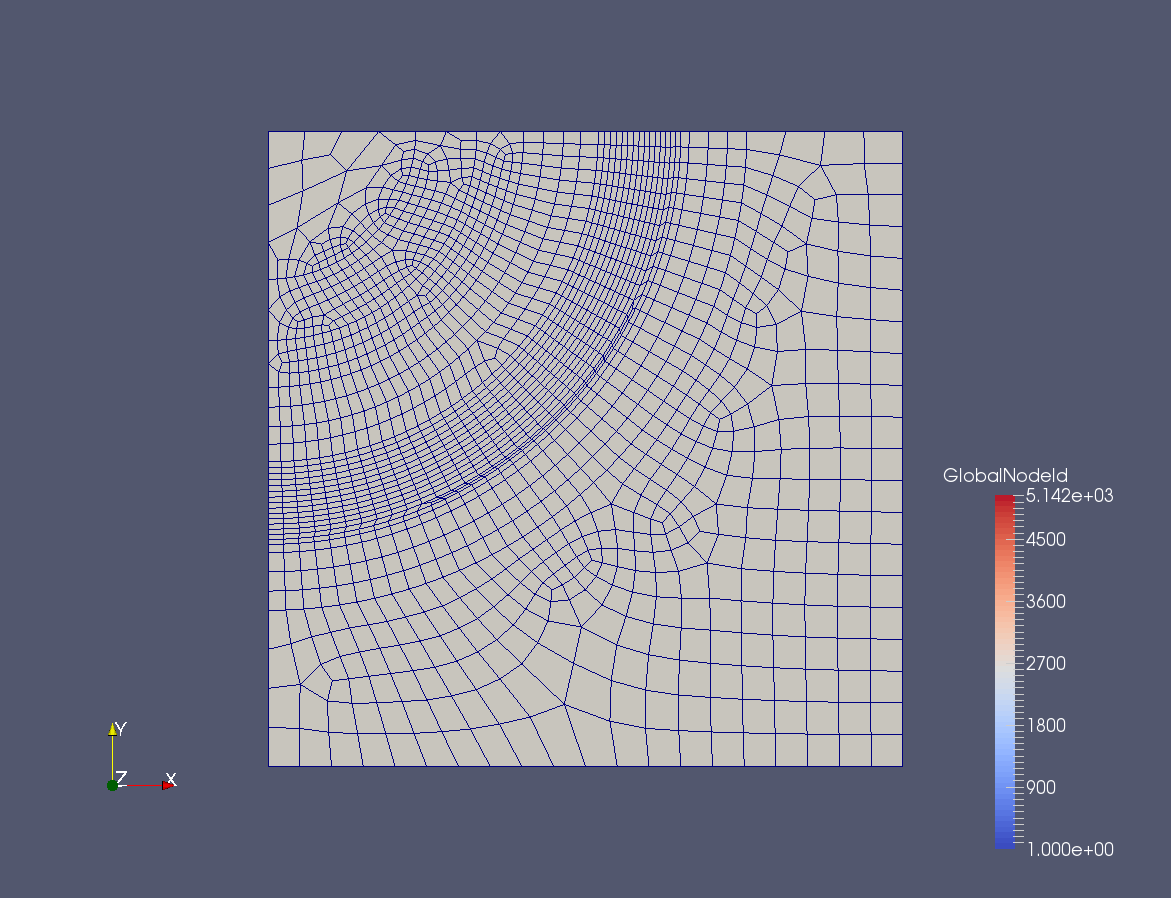
\includegraphics[width=0.7\linewidth]{pincell_mesh_png}
\end{figure}

The neutronics is calculated using 8 energy groups and takes as uncertain inputs 671 material cross
sections, including fission, capture, scattering, and neutron multiplication factor  Each cross section is
perturbed by 10\% of its original value, distributed normally.  The scattering cross
sections for each material in each group are not perturbed individually; rather, a scattering scaling factor
for each group is determined, and the scattering cross sections are all scaled by that factor.  The fission
and capture cross sections are perturbed individually.  The critical output of the neutronics calculation is
power shapes for use in the fuel performance code, as well as the $k$-eigenvalue for the rod.

The fuel performance code models mechanics such as heat conduction in the fuel, clad, and gap, clad stresses, grain radius
growth, and fuel expansion through the depletion steps of the fuel. The code takes power shapes
from the neutronics code as input and produces several key characteristics, such as peak clad temperature, maximum
fuel centerline temperature, and maximum clad stress.

The uncertain input space is highly correlated, so a Karhunen-Loeve (KL) component analysis is performed as
the first step in a two-part reduction \cite{physor2016}. The
covariance matrix is obtained via cross section construction in \texttt{scale}\cite{scale} using random sampling.  
Table \ref{tab:pcarank} gives the first several eigenvalues in the KL expansion.  Surrogate (or
\emph{latent}) dimensions identified by the KL expansion will be used as input variables for demonstration of
the various UQ methods.

\begin{table}[H]
  \centering
  \begin{tabular}{c|c}
Index & Eigenvalue \\ \hline
1 & 0.974489839965 \\
2 & 0.0183147250746 \\
3 & 0.00271597405394 \\
4 & 0.00260939137165 \\
5 & 0.000486257522596 \\
6 & 0.000431957645049 \\
7 & 0.000253683187786 \\
8 & 0.000228044411204 \\
9 & 0.000124030638175 \\
10 & 7.14328494102e-05 \\
11 & 6.30833696364e-05 \\
12 & 3.87071149672e-05 \\
13 & 3.51066363934e-05 \\
14 & 2.48699823434e-05 \\
15 & 1.98915286765e-05 \\
16 & 1.35985387253e-05 \\
17 & 1.128896325e-05 \\
18 & 9.59426898684e-06 \\
19 & 8.11612567548e-06 \\
20 & 7.16508951777e-06 \\
21 & 6.53366817241e-06 \\
22 & 4.50006575957e-06 \\
23 & 4.19287192651e-06 \\
24 & 3.7671309151e-06 \\
25 & 2.61683536224e-06 \\
26 & 2.22099981728e-06 \\
27 & 1.6360971709e-06 \\
28 & 1.13245742809e-06 \\
29 & 9.92282537141e-07
\end{tabular}
\caption{KL Expansion Eigenvalues for Pin Cell Problem}
\label{tab:pcarank}
\end{table}
 
% Chapter Template

\chapter{Methods} % Main chapter title

\label{Chapter3} % Change X to a consecutive number; for referencing this chapter elsewhere, use \ref{ChapterX}

\lhead{Chapter 3. \emph{Methods}} % Change X to a consecutive number; this is for the header on each page - perhaps a shortened title

%----------------------------------------------------------------------------------------
%	SECTION: INTRO
%----------------------------------------------------------------------------------------

\section{Todo}
todo.

% Chapter Template

\chapter{Preliminary Results} % Main chapter title

\label{ch:results} % Change X to a consecutive number; for referencing this chapter elsewhere, use \ref{ChapterX}

\lhead{Chapter 4. \emph{Results}} % Change X to a consecutive number; this is for the header on each page - perhaps a shortened title

We consider some results from applying the methods described in Chapter \ref{ch:methods} to the physical
models outlined in Chapter \ref{ch:models}, organized by model.
%----------------------------------------------------------------------------------------
%	SECTION 1
%----------------------------------------------------------------------------------------

\section{Polynomial Evaluations}
Using an analytic polynomial evaluation as our model allows observation of SCgPC performance for
multiple dimension cardinalities.  Uniformly distributing the input parameters from 0 to 1, the mean and variance are
\begin{align}
  \text{mean}&=\left(\frac{3}{2}\right)^N,\\
  \text{var}&=\left(\frac{7}{3}\right)^N-\left(\frac{3}{2}\right)^{2N},
\end{align}
where $N$ is the cardinality of the input space.  As seen in Figures \ref{fig:anl5_varconv} and
\ref{fig:anl10_varconv}, the increase in dimensionality has great impact on the convergence rate of SCgPC
methods.  There are several
inferences that we make using these results. In the figures, the following abbreviations are used:
\begin{itemize}
  \item \emph{mc}: Monte Carlo traditional sampling,
  \item \emph{tp}: Tensor Product-based SCgPC,
  \item \emph{td}: Total Degree-based SCgPC,
  \item \emph{hc}: Hyperbolic Cross-based SCgPC,
  \item \emph{adapt}: Adaptive SCgPC.
\end{itemize}

First, we note the tensor product (tp) method for polynomial basis set construction is an outlier, in that
with 200 computational solves the error is already converged to 11 orders of magnitude.  This is because of
the model being solved; it is, in effect, a tensor product of first-order polynomials.  For this particular
model, the tensor product method should be ideally efficient.  It is omitted in Fig.
\ref{fig:anl10_varconv} for clarity.

Second, we note that the two other static polynomial index sets, total degree (td) and hyperbolic cross (hc)
perform similarly well and converge faster than traditional Monte Carlo.  In the case of total degree, some
exponential convergence is observed, while it is unclear if hyperbolic cross is linear or exponential.  We
also note the strong dependence of SCgPC on input dimension cardinality for efficient convergence.

Finally, for this case we
also present some preliminary results for the Adaptive SCgPC method.  While it performs remarkably well for
the five-dimension problem, it stalls for the ten-dimension problem.  This is likely because of the
computational costs in searching the polynomial space.  Because of the tensor-first-order nature of the model,
the predictive algorithm behind Adaptive SCgPC incorrectly predicts that terms containing second-order
polynomials in any dimension are more significant than terms containing higher-interactivity first-order
polynomials.  Because of this, the Adaptive SCgPC method spends considerable effort in unproductive searching.

\begin{figure}[H]
  \centering
    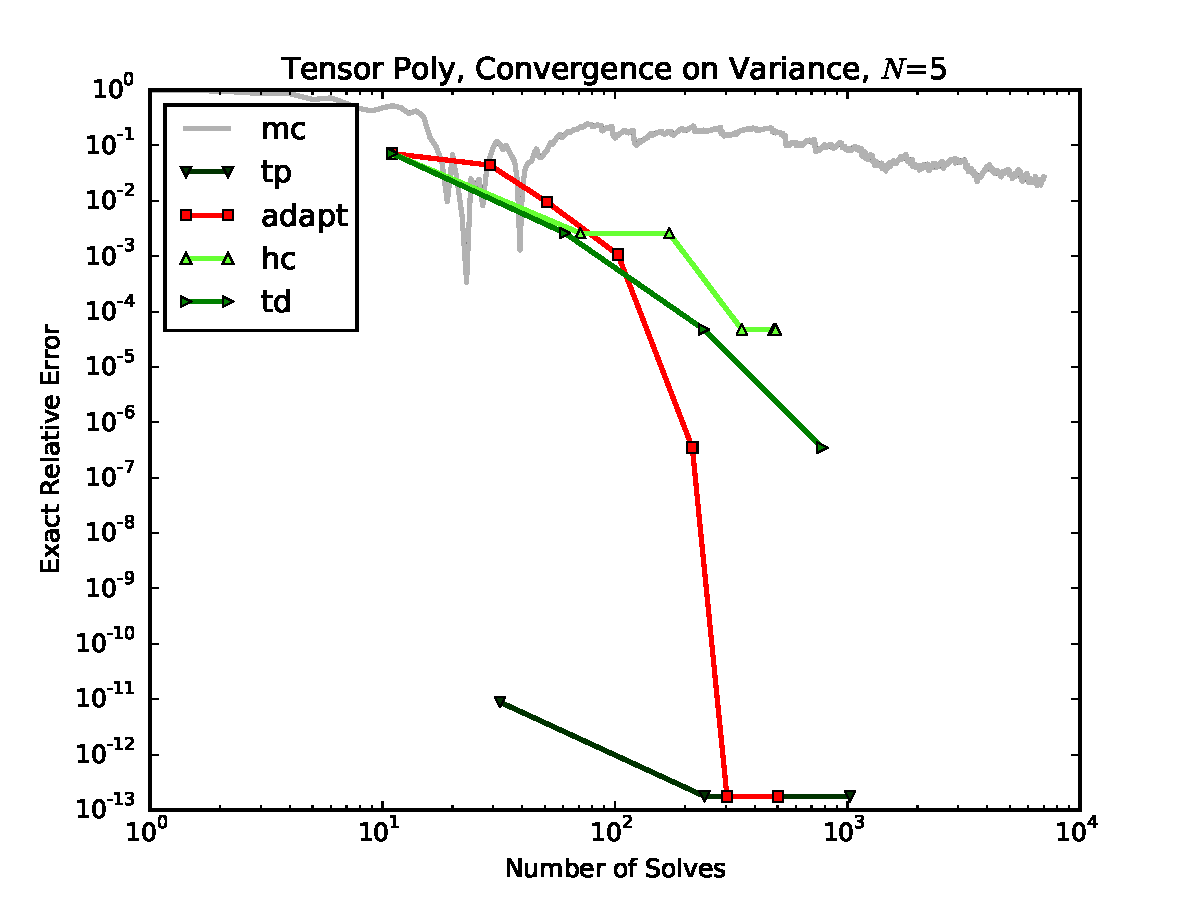
\includegraphics[width=0.7\linewidth]{tenspoly_varconv_5}
    \rule{35em}{0.5pt}
  \caption{Analytic $N=5$ Error Convergence, Variance}
  \label{fig:anl5_varconv}
\end{figure}
\begin{figure}[H]
  \centering
    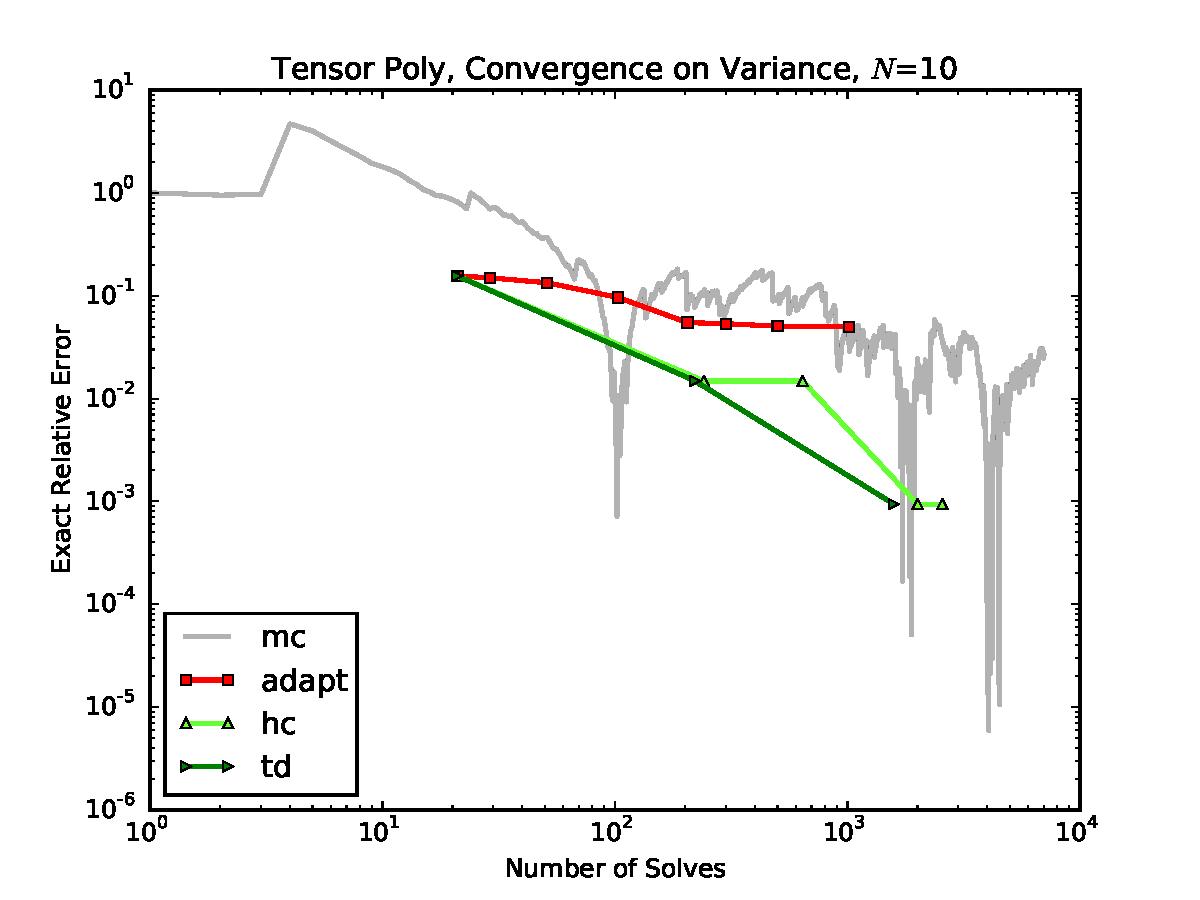
\includegraphics[width=0.7\linewidth]{tenspoly_varconv_10}
    \rule{35em}{0.5pt}
  \caption{Analytic $N=10$ Error Convergence, Variance}
  \label{fig:anl10_varconv}
\end{figure}



\section{Attenuation}
Similar to the polynomial model, the attenuation model does not converge exactly for any order of SCgPC
expansion, as exponential terms cannot be perfectly represented by a finite sum of polynomials.
Again distributing the input variables from 0 to 1, the mean and variance are
\begin{align}
  \text{mean}&=N^N\left(1-\exp(-\frac{1}{N})\right)^N,\\
  \text{var}&=\left(\frac{N}{2}\right)^N \left(1-\exp(-\frac{2}{N})\right)^N - \text{mean}^2,
\end{align}
where $N$ is the cardinality of the input space.  The convergence plots are shown in Figs.
\ref{fig:att5_varconv} and \ref{fig:att10_varconv}.

While considering this model, it is useful to expand the solution in a Taylor series for polynomial behavior.
In any one dimension,
\begin{equation}
  e^{-x} = 1 - x + \frac{x^2}{2!} - \frac{x^3}{3!} + \mathcal{O}(x^4).
\end{equation}
Because $y_n\in[0,1]$ and the nature of the polynomial expansion, we expect leading, low-order polynomial
terms to dominate the SCgPC expansion, and interactivity to be more dominant than high-order polynomials,
somewhat like the Polynomial Evaluations case above.

There are several notable features in this convergence graph that are not seen in the tensor polynomial case.
First, the Tensor Product and Total Degree index sets are very similar in exponential convergence; this is
somewhat expected given the polynomial expansions above.  Neither Total Degree nor Tensor Product ideally fit
this model as a low-order expansion, but both cover critical components of it as they grow in size.

The convergence of the Hyperbolic Cross index set is possibly the most striking result here.  The oscillatory
nature of the solutions covers a band wide enough to disguise any convergence after 100 computational solves.
It appears that the behavior is due to poor integration of high-order polynomial coefficients.  When a
polynomial is first added to the index set, insufficient quadrature is used to integrate the coefficient,
resulting in a large error for that coefficient.  However, when further points are added, the
poorly-integrated coefficient is resolved, and the variance converges more closely.  This behavior warrants
more investigation.

Lastly, we see some plateau behavior for the Adaptive SCgPC method. TODO WORKING XXX



Interestingly, while the convergence of the adaptive method seems to be converging at a better rate than the
total degree isotropic set, there is no clear advantage for up to thousands of solves.  This is somewhat
expected, as there is coupling between inputs evident in the Taylor expansion of the attenuation model.  
As with the polynomial model,
the curse of dimensionality is clear.

\begin{figure}[H]
  \centering
    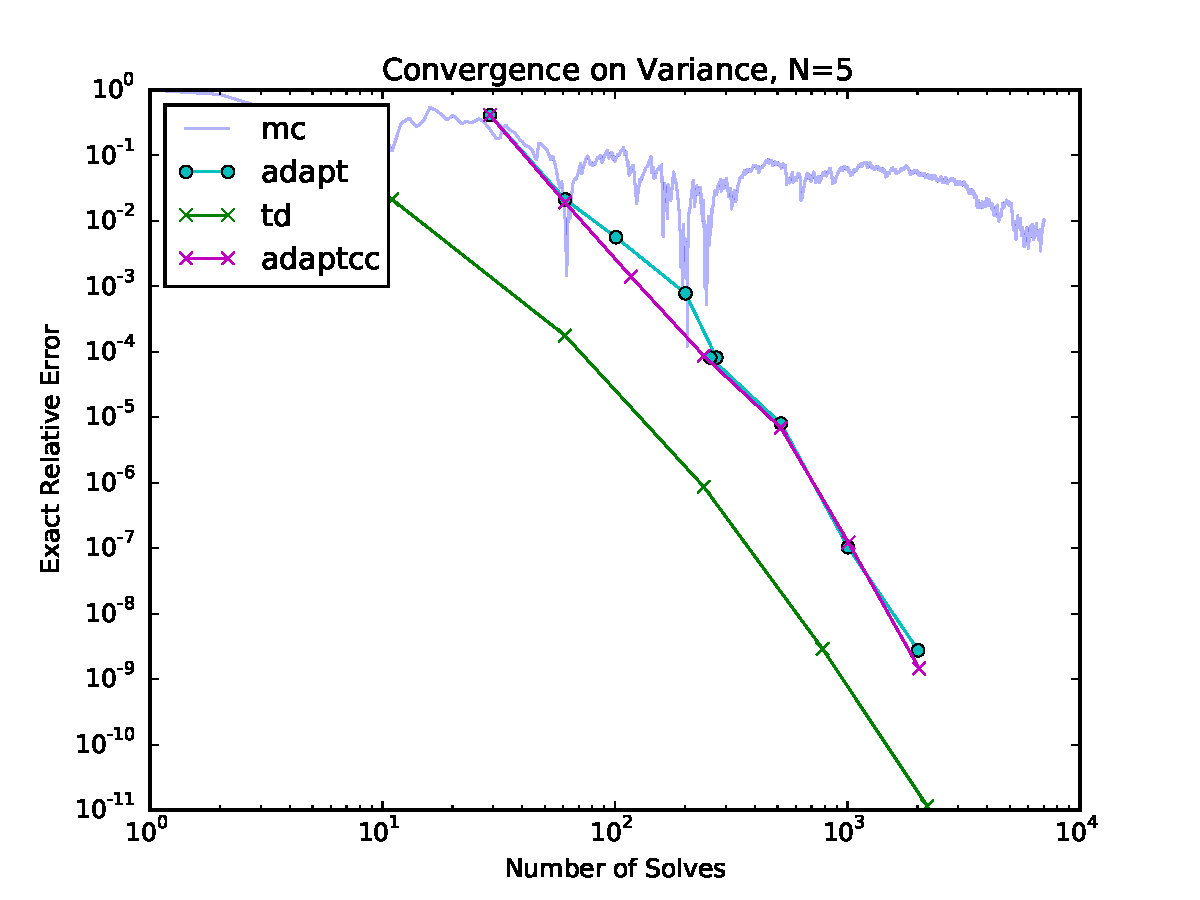
\includegraphics[width=0.7\linewidth]{attn_varconv_5}
    \rule{35em}{0.5pt}
  \caption{Attenuation $N=5$ Error Convergence, Variance}
  \label{fig:att5_varconv}
\end{figure}

\begin{figure}[H]
  \centering
    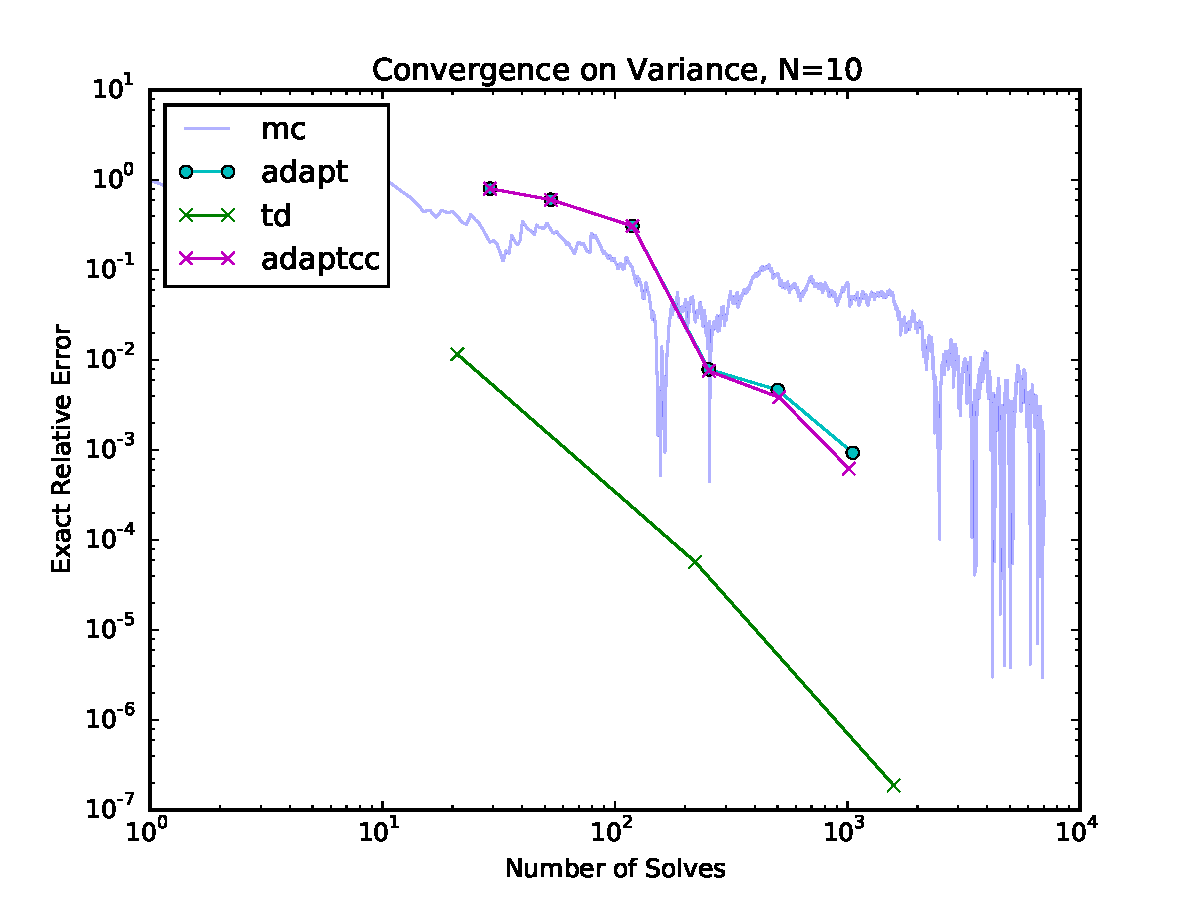
\includegraphics[width=0.7\linewidth]{attn_varconv_10}
    \rule{35em}{0.5pt}
  \caption{Attenuation $N=10$ Error Convergence, Variance}
  \label{fig:att10_varconv}
\end{figure}



\section{Projectile}
Unlike the attenuation and polynomial models, the projectile model is a nonlinear problem without an analytic
solution.  As a result, the convergence benchmark is one achieved by a large Monte Carlo run, instead of an
analytic benchmark; thus, the convergence of the various methods is limited to the convergence of the Monte
Carlo point.  The most converged Monte Carlo point for this work is
\begin{align}
  \text{mean} = 1234, \\
  \text{var} = 1234.
\end{align}
Additionally, this is the first model where significant anisotropy exists in the model.  For instance, the
drag coefficient parameter is many orders of magnitude more influential on the quantity of interest than the
gravitational acceleration.  
The results in Fig. \ref{fig:proj_varconv} are interesting, and require additional data points to understand
clearly.  However, we include Fig. \ref{fig:proj_varval} for clarity.  While it initially looks like the adaptive
methods converge quickly, it appears that this is misleading, as shown in the values graph.  The adaptive
method is converging, but passes through the benchmark value before turning back to converge on it.  This
indicates the adaptive construction introduces too much variance initially, and additional terms are required
to approach the benchmark solution.
\begin{figure}[H]
  \centering
    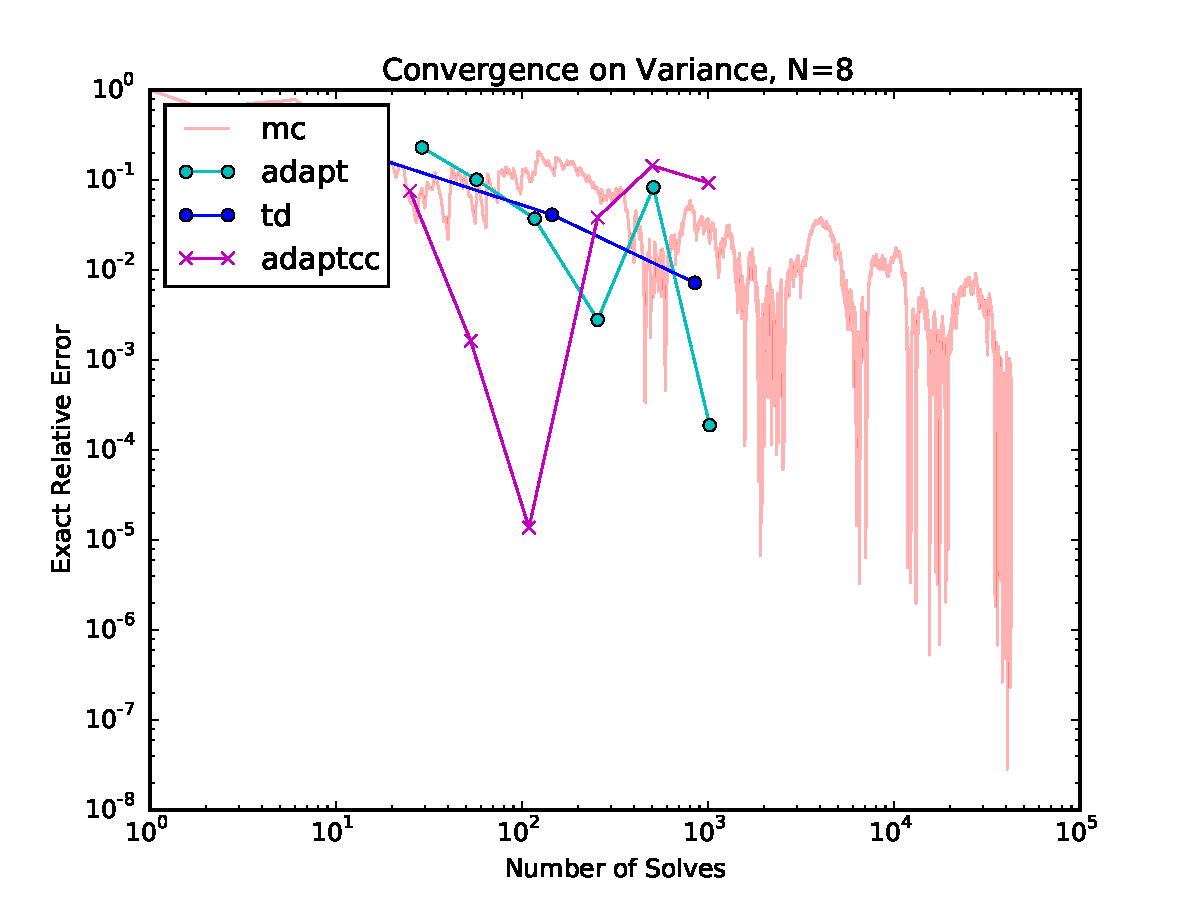
\includegraphics[width=0.7\linewidth]{proj_varconv_8}
    \rule{35em}{0.5pt}
  \caption{Projectile $N=8$ Error Convergence, Variance}
  \label{fig:proj_varconv}
\end{figure}
\begin{figure}[H]
  \centering
    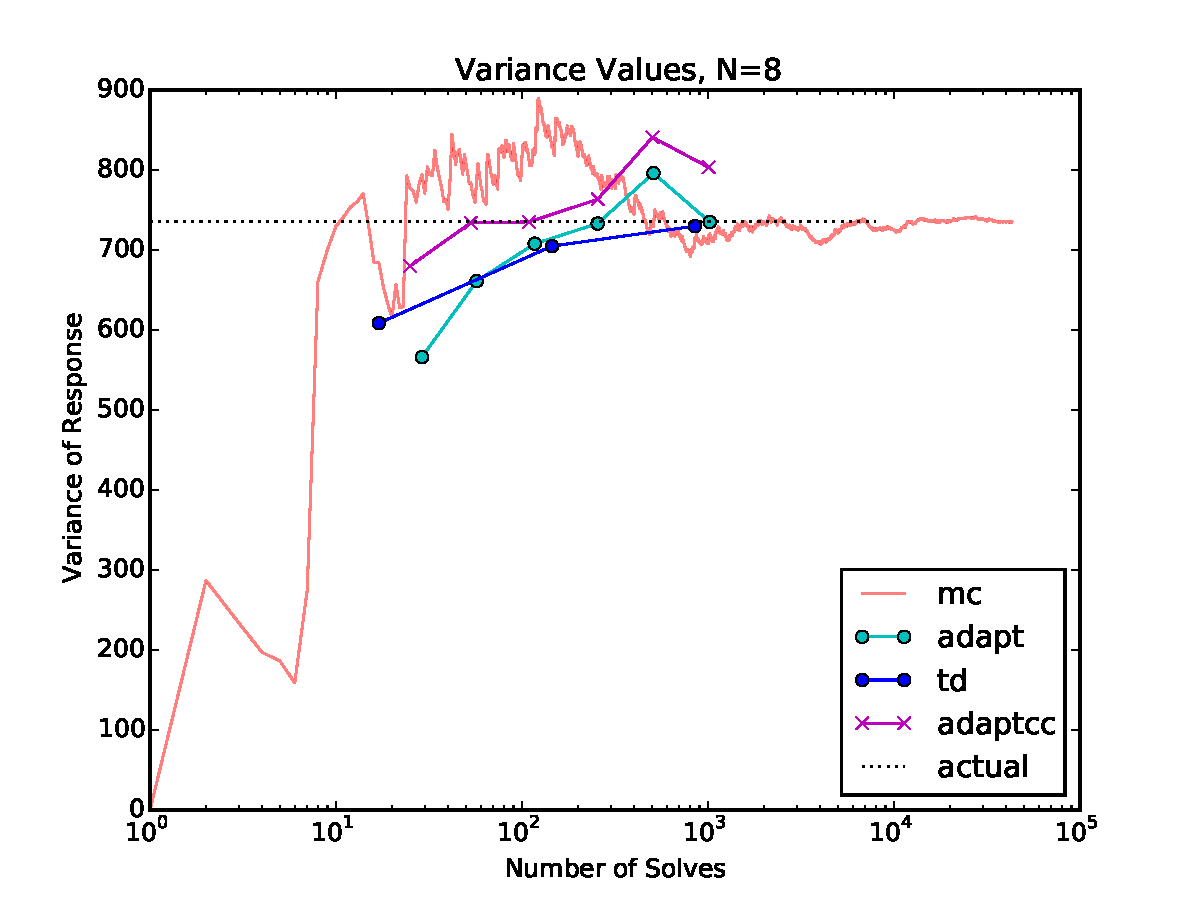
\includegraphics[width=0.7\linewidth]{proj_varvals_8}
    \rule{35em}{0.5pt}
  \caption{Projectile $N=8$ Values, Variance}
  \label{fig:proj_varval}
\end{figure}
%\begin{figure}[H]
% \centering
%   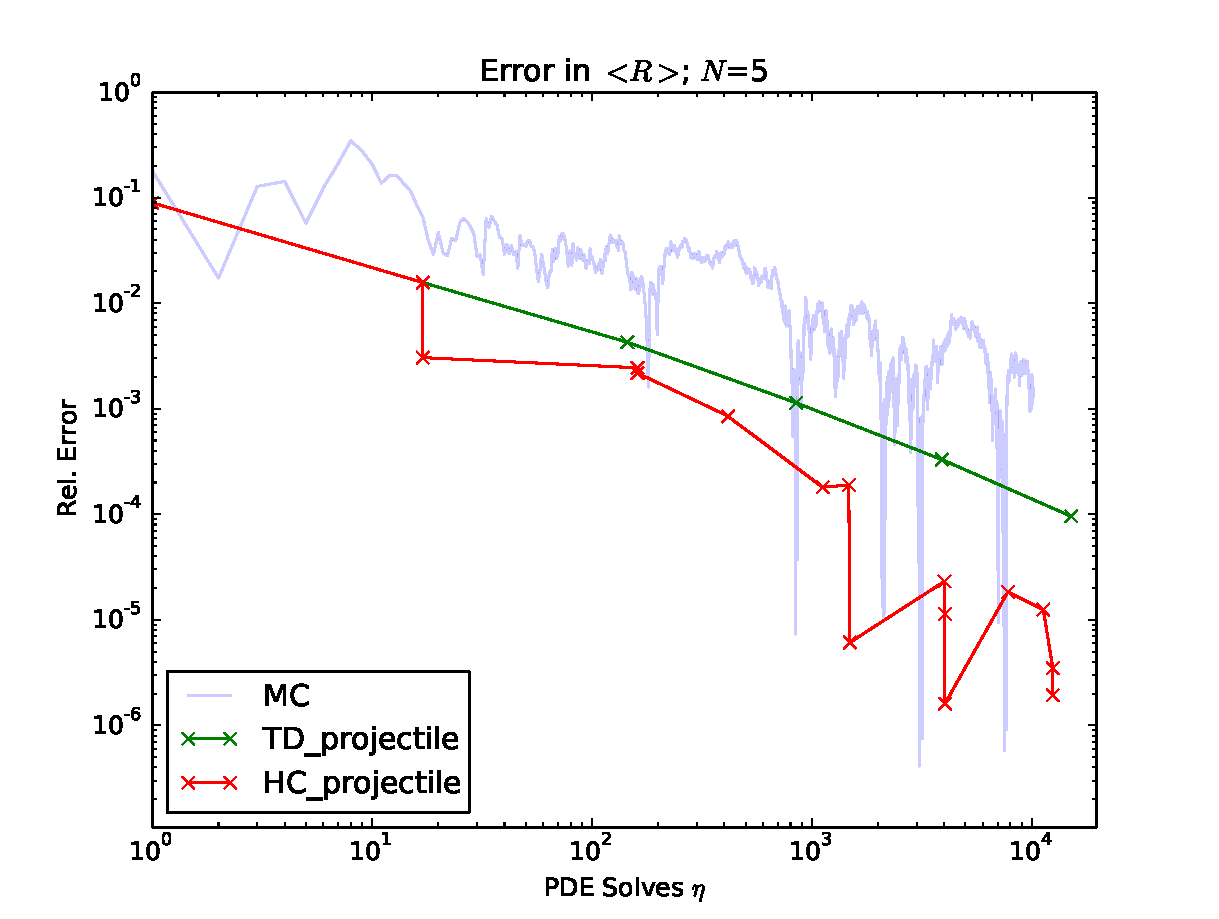
\includegraphics[width=0.7\linewidth]{projectile_errs}
%    \rule{35em}{0.5pt}
%  \caption{Projectile $N=8$ Error Convergence, Variance}
%  \label{fig:proj_varconv}
%\end{figure}



\section{Neutron Diffusion}
The neutron diffusion model is a complex, nonlinear model that begins to approach an engineering-scale model.
Because of complications with conflicting libraries, the adaptive SCgPC method was not available for this
model.  Particularly of note is the clear and obvious loss of convergence rate with increase in the
cardinality of the input space. \{Note to self: fix coloring in plots.\}

\begin{figure}[H]
  \centering
    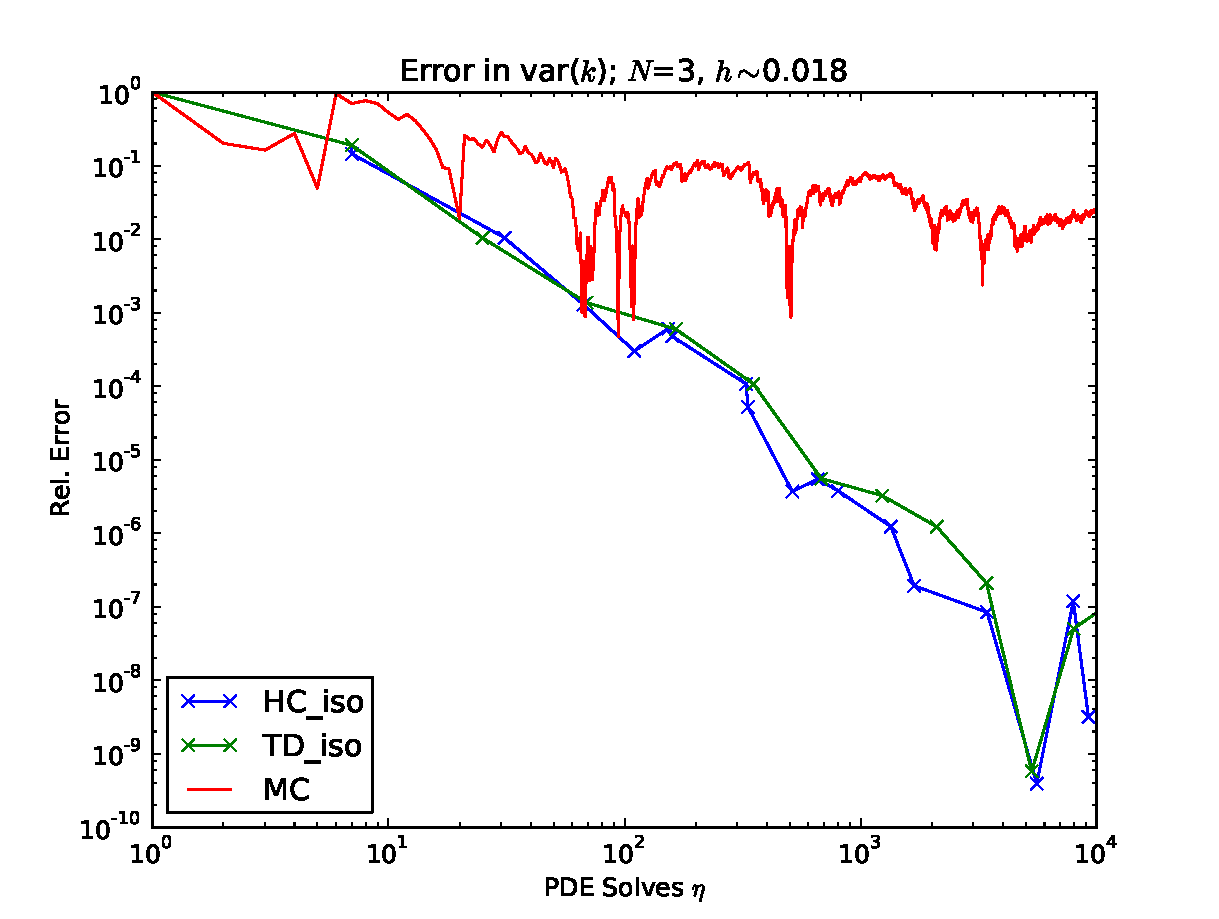
\includegraphics[width=0.7\linewidth]{N3_h5_MCHC_2}
    \rule{35em}{0.5pt}
  \caption{Diffusion $N=3$ Error Convergence, Variance}
  \label{fig:diff3_varconv}
\end{figure}
\begin{figure}[H]
  \centering
    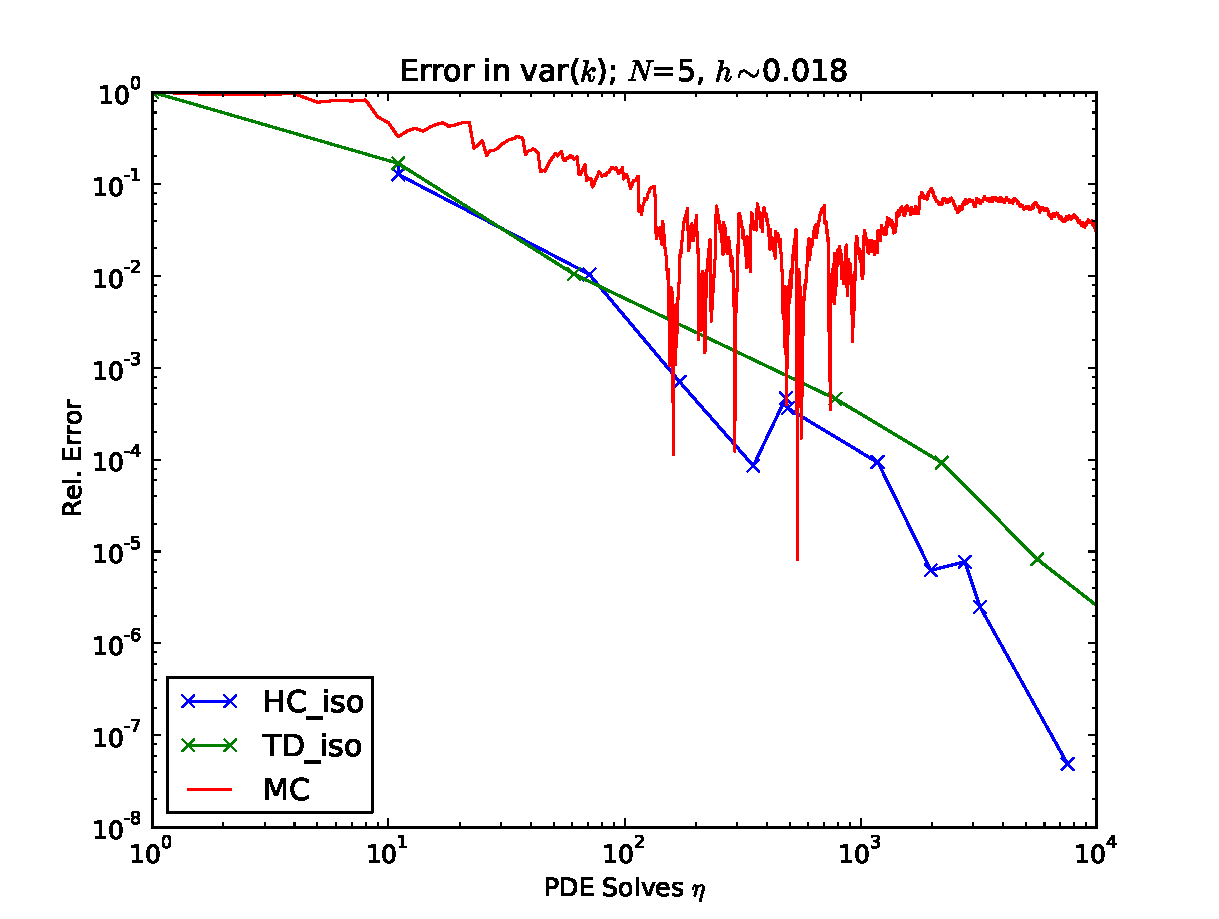
\includegraphics[width=0.7\linewidth]{N5_h5_MCHC_2}
    \rule{35em}{0.5pt}
  \caption{Diffusion $N=5$ Error Convergence, Variance}
  \label{fig:diff5_varconv}
\end{figure}
\begin{figure}[H]
  \centering
    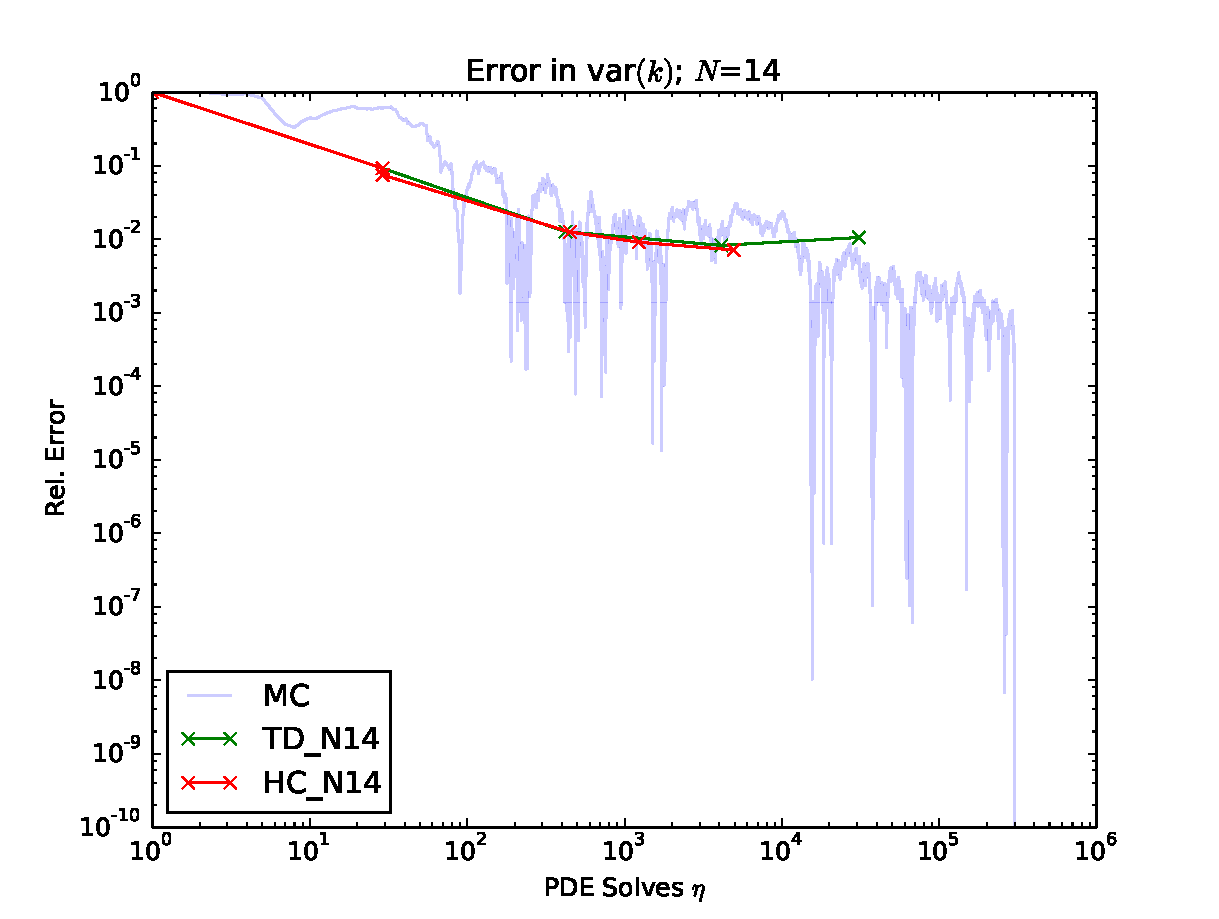
\includegraphics[width=0.7\linewidth]{N14_iso_var_errs}
    \rule{35em}{0.5pt}
  \caption{Diffusion $N=14$ Error Convergence, Variance}
  \label{fig:diff14_varconv}
\end{figure}





\section{Conclusions}
From evaluating the results using the various methods on these models, there are a few useful conclusions.

First, especially for models with small input cardinality, SCgPC methods tend to be faster converging than
traditional Monte Carlo methods.  In particular, the adaptive SCgPC method eventually exhibits exponential
convergence in the models considered here.  This is encouraging for many uncertainty quantification problems
where the variance is chiefly centered on a few input parameters.

%Second, using Clenshaw Curtis quadrature appears to have no negative consequence on converging with the
%adaptive SCgPC method, but no striking positive consequence either.  This suggests it is worth exploring other
%nested quadrature methods that might be beneficial in general, or at least in certain circumstances.

Second, it is clear that even with adaptive SCgPC, convergence is poor for input spaces with at least ten
inputs for less than a thousand solves.  For costly engineering codes, even a thousand runs may be
impractical, so further improvement of the adaptive algorithm is necessary.  This leads to the desirability of
the adaptive HDMR method, which can further subdivide the input domain.  These subdivided domains have
cardinality much more suitable to SCgPC methods.

Lastly, because SCgPC methods improve drastically with decreases in input cardinality, we expect SCgPC to
benefit from coupling with input reduction methods, such as sensitivity-weighted input reduction through
principal component analysis using input-input covariance matrices.
 
% Chapter Template

\chapter{Proposed Work} % Main chapter title

\label{ch:proposed} % Change X to a consecutive number; for referencing this chapter elsewhere, use \ref{ChapterX}

\lhead{Chapter 5. \emph{Proposed}} % Change X to a consecutive number; this is for the header on each page - perhaps a shortened title

Given the results in Chapter \ref{ch:results}, we consider the proposed work to complete as part of completing
degree work.

%----------------------------------------------------------------------------------------
%	SECTION 1
%----------------------------------------------------------------------------------------
\section{DRAFT NOTES}
\begin{itemize}
  \item I'm still updating the colors and contents of the results plots.  They'll be ready by January.
\end{itemize}

\section{Adaptive Sparse Grid}

There is a method proposed by \cite{Gerstner} and used in \cite{Ayres} whereby the polynomial index set to be
used in constructing the sparse grid quadrature is constructed adaptively.  We have demonstrated its
effectiveness in a preliminary manner in this work, but further improvements and demonstrations are critical
in exploring this method's potential.  The algorithm proceeds generally
as follows:
\begin{itemize}
  \item Begin with the mean (zeroth-order) polynomial expansion.
  \item While not converged:
    \begin{itemize}
      \item Collect a list of the polynomial index set whose predecessors have all been evaluated.
      \item Predict the impact of adding each polynomial to the existing polynomial index set.
      \item If the total impact of all indices is less than tolerance, convergence is reached.
      \item Otherwise, add the predicted highest-impact polynomial and loop back.
    \end{itemize}
\end{itemize}
This adaptive algorithm has the strength of determining the appropriate anisotropy to apply when generating a
polynomial index set.  For anisotropic cases, or cases where the static index set construction rules are not
ideal, the adaptive index set could potentially provide a method to avoid wasted calculations and emphasize
high-impact polynomials in the expansion.

PLACEHOLDER: VISUAL EXAMPLE OF 2D ADAPTIVE PROGRESSION

There are, however, some weak points in this algorithm.  First, the algorithm in literature has no predictive method
to determine the next polynomial index to include in the set; instead, it evaluates each potential index and
selects the one with the most impact \cite{Ayres}.  This is somewhat inefficient, because of SCgPC representations created
that are not used in the final product.  In addition to including this algorithm, we propose to develop a
method for predicting high-impact points based on the impact of their predecessors in the set.  Results shown
in this work are a first step in that direction.

Second, there are certain types of models for which the adaptive algorithm will stall, converge too early, or
otherwise generally fail.  For instance, if the partial derivative of the model with respect to any of the
input dimensions is zero when evaluated at the mean point (but nonzero elsewhere), the algorithm will falsely
converge prematurely, as adding additional polynomial orders to the input in question will not change the
value of the model at the mean point.  For example, consider a model
\begin{equation}
  f(a,b) = a^3b^3,
\end{equation}
with both $a$ and $b$ uniformly distributed on [-1,1].  We note the partial derivatives with respect to either
input variable evaluated at the central point (0,0) are zero.  The first polynomial index set point to
evaluate is zeroth-order in each dimension, [0,0].  We distinguish input domain points from polynomial index
set points by using parenthesis for the former and square brackets for the latter. The quadrature point to
evaluate this polynomial coefficient is (0,0), which, when evaluated, gives $f(0,0)=0$.  The next polynomial
index set combinations are [1,2] and [2,1].  For [1,2], the quadrature points required are
(0,$\pm\sqrt{1/3}$).  This evaluates to $f(0,\pm\sqrt{1/3})=0$, as well.  Because of symmetry, we obtain the
same result of [2,1].  According to our algorithm, because our old value was 0, and the sum of the new
contributions is 0, we have converged; however, we know this is false convergence.  While we expect few
applications for SCgPC to exhibit these zero partial derivatives in the input space, it is a limitation to be
aware of.  In addition to implementing this algorithm, we propose to find a way either to work around this
limitation, or at least to warn the user when such a case is likely to exist.


\section{Adaptive HDMR}
Despite the benefits of ideal anisotropic polynomial set construction promised by the adaptive SCgPC
algorithm, we expect the adaptive SCgPC to fall short for models where many input parameters provide relevant
uncertainty.  While the adaptive polynomial index set construction can preferentially emphasize particular
dimensions, it does not reduce the input cardinality of the problem.  An additional algorithm presented in
\cite{Ayres} uses an adaptively-constructed HDMR representation to alleviate the curse of dimensionality for
the adaptive SCgPC method.

In Chapter \ref{ch:methods}, we identify the static HDMR expansion, whereby subsets of the input domain can be
joined together to approximate the full model.  We replicate the essential expansion here:
\begin{align}
  u(Y) = u_0 &+ \sum_{n=1}^N u_{Y_n} \nonumber\\
  &+ \sum_{n_1=1}^N \sum_{n_2=1}^{n_1-1} u_{Y_{n_1},Y_{n_2}} \nonumber \\
  &+ \sum_{n_1=1}^N \sum_{n_2=1}^{n_1-1} \sum_{n_3=1}^{n_2-1} u_{Y_{n_1},Y_{n_2},Y_{n_3}} \nonumber \\
  &\cdots \nonumber\\
  &+u_{Y_{n_1},\cdots,Y_{n_N}},
\end{align}
where $u(Y)$ is the model, $Y$ is the combined input space, and $u_{Y_n}$ is an SCgPC surrogate model where
only $Y_n$ is considered varying and other input parameters are held at their reference value.  In static
HDMR, the desired largest subset size is selected, and all subset combinations are considered.  For instance,
for a model $f(a,b,c)$, the full HDMR expansion is
\begin{align}
  f(a,b,c,d) = f_0 &+ f_a + f_b + f_c \label{eq:exhdmr1}\\
    &+ f_{ab} + f_{ac} + f+{bc} \label{eq:exhdmr2}\\
    &+ f_{abc}. \label{eq:exhdmr3}
\end{align}
Truncating, a first-order HDMR expansion includes just the terms in Eq. \ref{eq:exhdmr1}, and a second-order
expansion additionally includes all the terms in Eq. \ref{eq:exhdmr2}.  However, it is entirely possible and
often likely that
some subsets have larger impact than others, and some might be ignored altogether without significantly
impacting the overall expansion.  Adaptive HDMR (AHDMR) is an algorithm that considers the potential impacts
of adding new polynomials to existing subsets (as in the Adpative Sparse Grid algorithm) as well as the
potential impact of adding new subsets to the HDMR expansion. The AHDMR algorithm proceeds as follows:
\begin{itemize}
  \item Evaluate the reference (all mean) case.
  \item Construct all first-order expansion surrogate models.
  \item While not converged:
  \begin{itemize}
    \item Using existing subset sensitivities, predict the importance of future subsets
    \item Consider the impact of adding polynomial indices to existing subset PCE representations.
    \item Choose between expanding existing subsets or adding new subsets based on impact.
    \item If the relative contribution of the new HDMR expectation is less than tolerance, convergence is reached.
  \end{itemize}
\end{itemize}
All the surrogate models for each subtype in the expansion are constructed using adaptive SCgPC expansions.
Because the input space for the subset surrogates is small, and grows slowly as the method progresses, they
are ideally suited for SCgPC methods.  However, we note that any surrogate model, or the original model
itself, can be used instead of adaptive SCgPC reduced-order models.

For the case demonstrated by \cite{Ayres}, combining adaptive HDMR and adaptive SCgPC makes it possible to
compete in convergence with Monte Carlo for input spaces with cardinality nearly up to a thousand.  Adding
more efficient polynomial index set choices for adaptive SCgPC, we expect to see additional increases in 
performance.

\section{Quadrature}
The numerical integrations in this work have all been performed using classic Gaussian quadrature sets
(Legendre, Hermite, Laguerre, Jacobi).  It is also possible to use other quadrature sets for integration, such
as Clenshaw-Curtis or Gauss-Patterson.  These quadratures have the benefit of nested quadratures when chosen
correctly, which, especially for adaptive methods, can save considerable computation.  We propose to implement
at least one of these nested quadratures and contrast the performance of SCgPC methods using both classic and
nested quadratures.

\section{Engineering Application}
Lastly, we propose to implement all of the methods discussed here in production-scale uncertainty
quantification code \raven{}, and apply them in quantifying the uncertainty of a nonlinear multiphysics
problem.  In particular, we propose considering a two-dimensional quarter-pin cell nuclear engineering problem
coupling \moose{} applications \rattlesnake{}, a neutron transport code, and \bison{}, a fuel performance
code.
 
%\input{Chapters/Chapter6} 

%----------------------------------------------------------------------------------------
%	THESIS CONTENT - APPENDICES
%----------------------------------------------------------------------------------------

%\addtocontents{toc}{\vspace{2em}} % Add a gap in the Contents, for aesthetics

%\appendix % Cue to tell LaTeX that the following 'chapters' are Appendices

% Include the appendices of the thesis as separate files from the Appendices folder
% Uncomment the lines as you write the Appendices

%% Appendix A

\chapter{Appendix Title Here} % Main appendix title

\label{AppendixA} % For referencing this appendix elsewhere, use \ref{AppendixA}

\lhead{Appendix A. \emph{Appendix Title Here}} % This is for the header on each page - perhaps a shortened title

Write your Appendix content here.
%\input{Appendices/AppendixB}
%\input{Appendices/AppendixC}

%\addtocontents{toc}{\vspace{2em}} % Add a gap in the Contents, for aesthetics

\backmatter

%----------------------------------------------------------------------------------------
%	BIBLIOGRAPHY
%----------------------------------------------------------------------------------------

\label{Bibliography}

\lhead{\emph{Bibliography}} % Change the page header to say "Bibliography"

\bibliographystyle{unsrtnat} % Use the "unsrtnat" BibTeX style for formatting the Bibliography

\bibliography{Bibliography} % The references (bibliography) information are stored in the file named "Bibliography.bib"

\end{document}
